\title{Warm-Up for April 18th, 2022}
\author{Dr. Jordan Hanson - Whittier College Dept. of Physics and Astronomy}
\date{\today}
\documentclass[12pt]{article}
\usepackage[a4paper, total={18cm, 27cm}]{geometry}
\usepackage{graphicx}
\usepackage{amsmath}
\usepackage{subcaption}
\usepackage{bm}
\def\rcurs{{\mbox{$\resizebox{.16in}{.08in}{
\includegraphics{ScriptR}}$}}}
\def\brcurs{{\mbox{$\resizebox{.16in}{.08in}{
\includegraphics{BoldR}}$}}}
\def\hrcurs{{\mbox{$\hat \brcurs$}}}
 
\begin{document}
\maketitle
\small
\section{Memory Bank}
\begin{enumerate}
\item Recall that $\mathbf{a} = \int_{\mathcal{S}} d\mathbf{a} = \mathbf{a}$ is the vector area of a surface, and that if $\mathbf{c}$ is some constant vector:
\begin{equation}
\oint (\mathbf{c} \cdot \mathbf{r}) d\mathbf{l} = \mathbf{a} \times \mathbf{c} \label{eq:1}
\end{equation}
\item Let $\mathbf{c} = \hat{\mathbf{r}}$, and reverse the order of the cross-product:
\begin{equation}
\oint (\hat{\mathbf{r}} \cdot \mathbf{r}') d\mathbf{l}' = -\hat{\mathbf{r}} \times \int d\mathbf{a}' \label{eq:2}
\end{equation}
\item The \textit{magnetic multipole expansion} for a line current $I$ is
\begin{equation}
\mathbf{A}(\mathbf{r}) = \frac{\mu_0 I}{4\pi} \oint \frac{1}{\rcurs}d\mathbf{l}' = \frac{\mu_0 I}{4\pi} \sum_{n=0} \frac{1}{r^{n+1}} \oint (r')^n P_n (\cos\alpha) d\mathbf{l}'
\end{equation}
\end{enumerate}

\section{Magnetic Multipole Expansion}

\begin{enumerate}
\item In the magnetic multipole expansion, set $n=0$ with $P_1(\cos\alpha) = 1$ to calculate the monopole term. Why is it zero? \\ \vspace{1cm}
\item In the magnetic multipole expansion, set $n=1$ with $P_1(\cos\alpha) = \cos\alpha$.  Using Eq. \ref{eq:2}, with $\cos\alpha = \hat{\mathbf{r}} \cdot \mathbf{r}'$ (Fig. \ref{fig:1}), show that 
\begin{equation}
\mathbf{A}_{dipole}(\mathbf{r}) = \frac{\mu_0}{4\pi}\frac{\mathbf{m} \times \hat{\mathbf{r}}}{r^2}
\end{equation}
The vector $\mathbf{m}$ is a constant, the \textit{magnetic dipole moment.} What is its definition?
\end{enumerate}

\begin{figure}
\centering
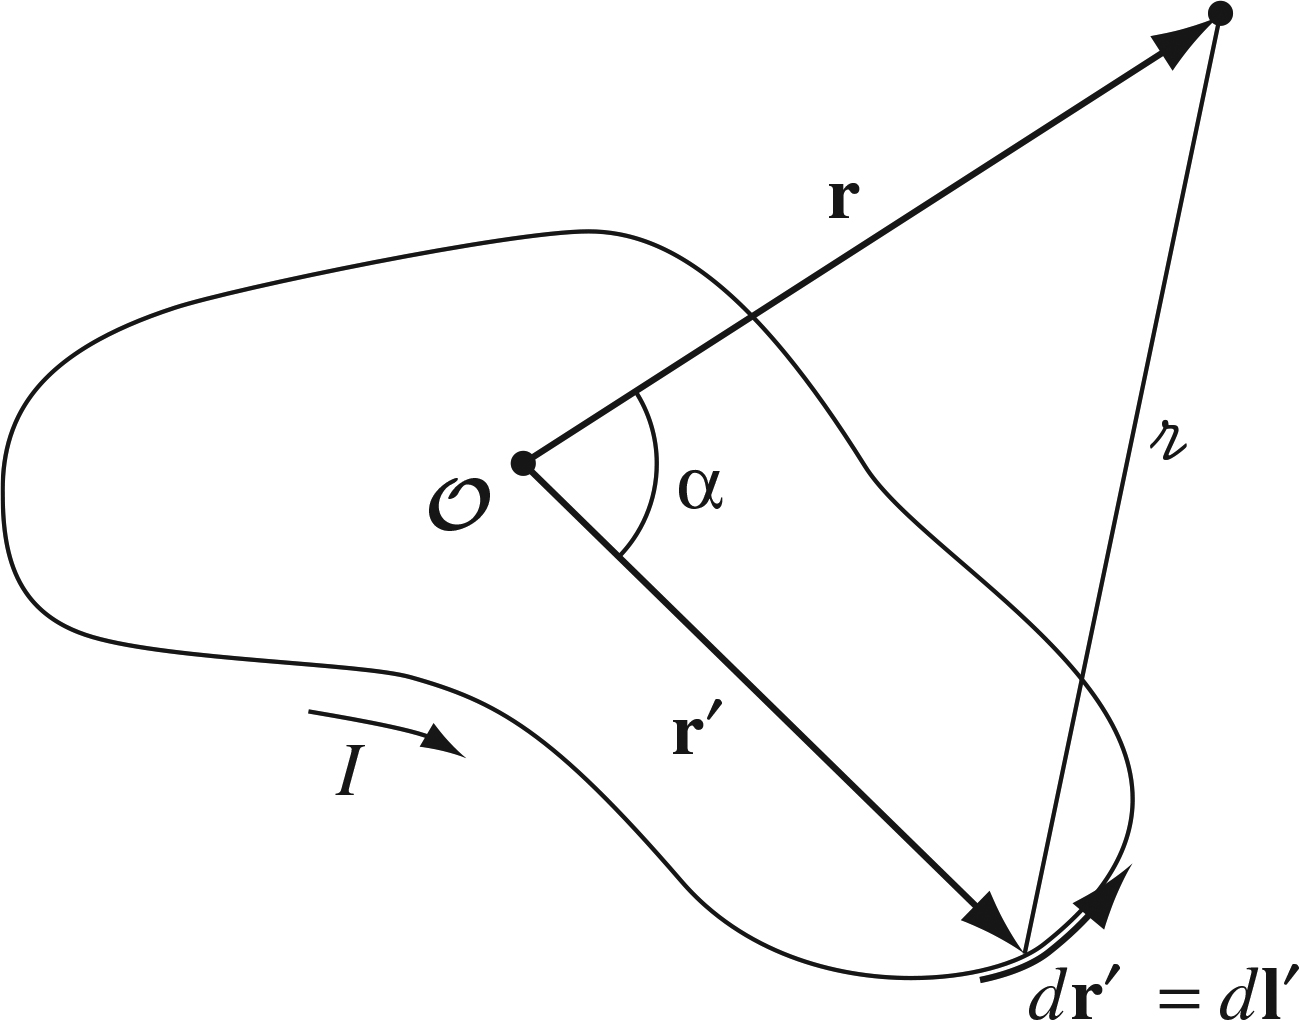
\includegraphics[width=0.25\textwidth]{figures/5_51.jpg}
\caption{\label{fig:1} A line current of strength $I$ and observed at displacement $\rcurs$.}
\end{figure}

\end{document}